\lfoot{Autor: Daniel Melichar}
\subsubsection{Nicht relationale Datenbanken (NoSQL)}
\label{subsec:nichtrelationaleDB}

In diesem Kapitel wird ein Einblick in das Konzept von nicht-relationalen Datenbanken gegeben. 

\paragraph{Motive und Beweggründe}\mbox{}\\
Der Term \textit{NoSQL} wurde erstmalig 1998 für eine relationale Datenbank, welche ohne der SQL-Sprache funktioniert, verwendet \cite{MELD.CH2-noSQL.firstSQLNaming}. Der Term wurde dann immer wieder über die Jahre von verschiedensten Leuten aufgenommen. Unglücklicherweise gab es keine definitive Beschränkung dafür, welche Datenbanksysteme zur NoSQL-Bewegung gehören. Durch den Blogger und Rackspace Mitarbeiter, Eric Evans, ist der Term ganz besonders bekannt geworden – er sagte hierzu: \textit{“the whole point of seeking alternatives is that you need to solve a problem that relational databases are a bad fit for”} \cite{MELD.CH2-noSQL.whatsInAName}. NoSQL Datenbanken wurden hauptsächlich von Großkonzernen für den Eigenbedarf entwickelt (Amazon’s Dynamo, Google’s BigTable, LinkedIn’s Voldemort, Facebook’s Cassandra, Yahoo!’s PNUTS). Diese Großkonzerne haben den relationalen Ansatz nicht komplett verworfen, sie fanden lediglich, dass das Modell nicht ihren Anforderungen entspricht \cite{MELD.CH2-noSQL.capTheoremComp}.

Das bekannte IT und Technologie Magazin \textit{Computerworld} hat im Jahre 2009 bei einer NoSQL Konferenz in San Franciso die dort vorhanden Developer befragt, wieso NoSQL gegenüber relationalen Datenbanken im Vorteil ist \cite{MELD.CH2-noSQL.whyItsBetter}.

Die folgenden Erklärungen wurden von den Entwicklern geliefert.
\begin{itemize}
	\item \textbf{Unnötige Komplexität wird vermieden}\newline
	 Relationale Datenbanken verfügen über eine große Anzahl an Features und strikten Bestimmungen bei Datenkonsistenz. Jedoch kann diese Anzahl an Features und die Anbindung an das ACID-Model zu viel für spezifische Anwendungsfälle sein. Zum Beispiel ist die Überprüfung von Session Daten, die mehrmals als Kopie abgespeichert sind, nicht notwendig.

	\item \textbf{Hohe Verarbeitungsmenge}\newline
	 Manche NoSQL Datenbanken erlauben einen höheren Datendurchsatz, bzw. eine schnelleren Verarbeitungsgeschwindigkeit. Die Möglichkeit, einfach und schnell eine neue Maschine in das System anzubinden, und somit mehr Rechenleistung zu erhalten, ist vom großen Vorteil.

	\item \textbf{Horizontale Skalierbarkeit und geringe Hardware requirements}\newline
	 Im Vergleich mit relationalen DBMS, sind die meisten NoSQL Datenbanken konzipiert, um horizontale Skalierung möglichst einfach durchzuführen. Horizontale Skalierung bedeutet prinzipiell: mehr Server in den Pool der Ressourcen hinzuzufügen. Es gibt zwar auch eine äquivalente Verbesserungsmöglichkeiten für RDBMS, das so genannte \textit{sharding}, die Umsetzung ist aber, aus persönlicher Erfahrung, um einiges komplizierter als bei NoSQL.

	\item \textbf{Object-Relational Mapping wird vermieden}\newline
	 Die meisten NoSQL Datenbanken verwenden eine Struktur zur Speicherung der Daten, die entweder sehr einfach oder sehr ähnlich zu jenen sind, welche auch bei Objekt-Orientierten-Programmiersprachen aufzufinden sind. Hierfür ist dann kein ressourcenintensives Object-Relational Mapping notwendig.
\end{itemize}

Zu diesem Bericht gab es dann auch einen Blog-Eintrag von Nati Shalom, CTO und Gründer von GigaSpaces. Er hat die folgenden weiteren Punkte für die NoSQL-Bewegung aufgestellt \cite{MELD.CH2-noSQL.natiShalomlol}.

\begin{itemize}
	\item \textbf{Komplexität und benötigter Aufwand der Datenbank Clustern}\newline
	 Er meint, dass NoSQL Datenbanken auf eine Art und Weise entwickelt worden sind, welche die Erstellung von Clustern sehr einfach macht. Unter anderem spielt hier auch das bereits angesprochene Skalieren auf horizontaler Ebene eine große Rolle.
	
	\item \textbf{Kompromiss zwischen Performance und Verlässlichkeit}\newline
	 Shalom behauptet außerdem, dass es verschiedene Szenarien gibt, in welchen Applikationen den Fokus auf Performance legen und nicht auf Verlässlichkeit. Ein gutes Beispiel für dieses Szenario sind die Daten von HTTP Sessions – diese müssen zwischen vielen Web Servern verteilt werden, löschen sich aber dann sobald der User sich abmeldet.

	\item \textbf{Cloud Computing}\newline
	 Hier werden sehr oft NoSQL Lösungen verwendet, da das Limit der Skalierbarkeit sehr hoch, bis sogar unendlich ist. Es müssen auch wenig administrative Tätigkeiten im Umgang mit NoSQL durchgeführt werden und es gubt viele NoSQL Datenbanken, die spezifisch für Datawarehousing entwickelt worden sind.
\end{itemize}

\paragraph{Techniken und Konzepte}\mbox{}\\
\textbf{Das CAP-Theorem\newline}
\label{subsec:captheor}
Das von Eric Brewer im Jahre 2000 entwickelte CAP-Theorem stellt eine Behauptung über die möglichen Fähigkeiten eines DBMS auf. Der CAP Akronym steht für \cite{MELD.CH2-noSQL.capTheorem}:

\begin{itemize}
	\item \textit{Consistency:} Ob und wie ein System in den konsistenten Zustand, nach Ausführung einer Operation, zurück gelangt. Ein verteiltes System wird im Normalfall als Konsistent bezeichnet, wenn alle lesenden Teile das selbe Resultat aus dem geteilten Informationspool bekommen.

	\item \textit{Availability:} Hierbei ist vor allem auf das Design und die Umsetzung eines Systems zu achten. Es sollte so entwickelt sein, dass bei Ausfall eines Servers in einem Cluster, immer noch die selben Operationen durchgeführt werden können.

	\item \textit{Partition Tolerance:} Anders als bei Availability geht es hier meistens um Netzwerk Partitionen und die Möglichkeit weiter Operationen durchzuführen, wenn zwei Netzwerke im System nicht miteinander kommunizieren können.
\end{itemize}

 Brewer behauptet, dass nur zwei von diesen drei Eigenschaften in einem \textit{shared-data system} vorhanden sind \cite{MELD.CH2-noSQL.capTheorem}. In seiner Präsentation hat er über die Vor- und Nachteile von ACID und BASE Systemen (siehe Paragraphe \ref{subsec:acidvsbase}) geredet und einige Entscheidungskriterien vorgestellt um sich für eine der beiden Modelle zu entscheiden: wenn ein System, oder Teile eines Systems, konsistent und partitionstolerant sein müssen, werden ACID Eigenschaften benötigt; wenn Verfügbarkeit und Toleranz gegenüber Teilung bevorzugt werden, sollte das System mittels BASE Eigenschaften erstellt werden. Anhand Tabelle \ref{table:capTheorChoice} lassen sich die Zusammenhänge am besten veranschaulichen.

\begin{table}[!htb]
\centering
\begin{tabular}{|l|l|l|}
\hline
\multicolumn{1}{|c|}{\textbf{Choice}} & \multicolumn{1}{c|}{\textbf{Traits}} & \multicolumn{1}{c|}{\textbf{Examples}} \\ \hline
Consistence + Availability & \begin{tabular}[c]{@{}l@{}}2-phase-commit\\ cache-validation protocols\end{tabular} & \begin{tabular}[c]{@{}l@{}}Single-site databases\\ Cluster databases\\ LDAP\\ xFS file system\end{tabular} \\ \hline
Consistency + Partition tolerance & \begin{tabular}[c]{@{}l@{}}Pessimistic locking\\ Make minority partions unavailable\end{tabular} & \begin{tabular}[c]{@{}l@{}}Distributed databases\\ Distributed locking\\ Majority protocols\end{tabular} \\ \hline
Availability   + Partition tolerance & \begin{tabular}[c]{@{}l@{}}expirations/leases\\ Conflict resolution\\ Optimistic\end{tabular} & \begin{tabular}[c]{@{}l@{}}Coda\\ Web caching\\ DNS\end{tabular} \\ \hline
\end{tabular}
\caption{CAP-Theorem – Alternatives, Traits, Examples \cite{MELD.CH2-noSQL.capTheorem}}
\label{table:capTheorChoice}
\end{table}

Grundsätzlich kann gesagt werden, dass RDBMS besser Anforderungen nach Konsistenz und Teilungstoleranz abdecken und NoSQL-Systeme vornehmlich auf eine hohe Verfügbarkeit abzielen (siehe Abbildung \ref{fig:captheor}) \cite{MELD.CH2-noSQL.capTheoremComp}.

\begin{figure}[!htb]\centering
	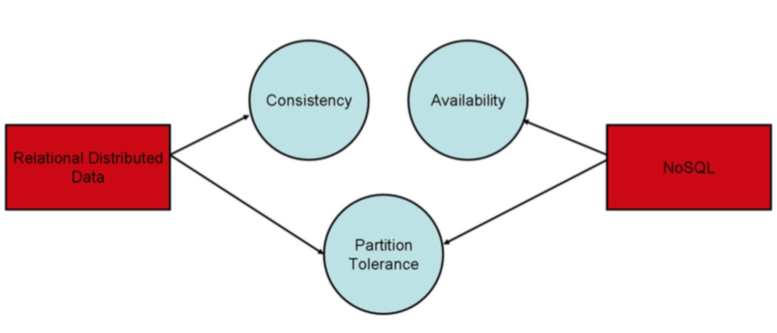
\includegraphics[width=0.8\textwidth]{images/capTheorem}
	\caption{CAP-Theorem bei RDBMS und NoSQL \cite{MELD.CH2-noSQL.capTheoremComp}}
	\label{fig:captheor}
\end{figure}

\clearpage

\label{subsec:acidvsbase}
\textbf{ACID vs BASE\newline}
Applikationen haben einen unterschiedlichen Bedarf an Performance, Zuverlässigkeit, Betriebsbereitschaft, und Konsistenz. Wie bereits beim CAP-Theorem beschrieben (\ref{subsec:captheor}) können Applikationen nur zwei Optionen von Consistency, Availability, und Partition Tolerance besitzen. Für die stetige Weiterentwicklung von NoSQL-Systemen, welche die Option von Availability und Partition Tolerance implementieren, wurde ein ACID ähnliches Modell entwickelt.

Das Akronym BASE steht für folgende Eigenschaften
\begin{itemize}
	\item Basically Available
	\item Soft-state
	\item Eventual consistency
\end{itemize}

Tabelle \ref{table:acidvsbase} stellt Eric Brewers Vergleich zwischen ACID und BASE dar. Es ist jedoch zu beachten, dass diese beiden Konzepte sich nicht aufheben, sondern ein großes Spektrum an Möglichkeiten bieten sollen. 

\begin{table}[!htb]
\centering
\label{acidvsbaseTable}
\begin{tabular}{|l|l|}
\hline
\multicolumn{1}{|c|}{\textbf{ACID}} & \multicolumn{1}{c|}{\textbf{BASE}} \\ \hline
\begin{tabular}[c]{@{}l@{}}Strong consistency \\ Isolation \\ Focus on “commit” \\ Nested transactions \\ Availability? \\ Conservative (pessimistic) \\ Difficult evolution (e.g. schema)\end{tabular} & \begin{tabular}[c]{@{}l@{}}Weak consistency – stale data OK \\ Availability first\\ Best effort \\ Approximate answers OK \\ Aggressive (optimistic)\\ Simpler!\\ Faster \\ Easier evolution\end{tabular} \\ \hline
\end{tabular}
\caption{Eric Brewer:ACID vs BASE  \cite{MELD.CH2-noSQL.capTheorem}}
\label{table:acidvsbase}
\end{table}

\textbf{Partitionierung\newline}
Ein weiteres, von relationalen DBMS abgeleitetes Konzept ist die gezielte Trennung der Daten auf mehreren Maschinen. Ab einer gewissen Menge an Daten werden die benötigten Ressourcen über die Kapazität einer einzelnen Maschine hinaus laufen. In diesem Fall müssen die Daten über mehrere Maschinen aufgeteilt werden – dies ist als \textit{Partitioning} bekannt. Hierbei gilt es auch zu beachten, dass  das System weiterhin funktionsfähig sein muss, wenn einer dieser Maschinen ausfällt. Es sollte auch beachtet werden, dass die Ressourcen auf alle Server gleich aufgeteilt ist (\textit{load balancing}).

Bei NoSQL Datenbanken gibt es hierfür verschiedene Konzepte um die bestmöglichen Ergebnisse zu erhalten.

\begin{description}
	\item[Memory Caches] können als separate Zwischenspeicher (z.B. RAM) Datenbanken gesehen werden. Hierbei werden die am meisten gebrauchten Daten mit einer hohen Frequenz in den Memory gespeichert und somit eine Art von Caching entwickelt. In den meisten Fällen werden die Daten über eine API und einen speziellen Key geholt.

	\item[Clustering] von Datenbanken ist eine weitere Möglichkeit. Es werden hier mehrere Server in komplexen Netzwerkstrukturen verknüpft. Es ist vor allem sehr wichtig, dass der Verwender der Applikation gar nicht mitbekommt, mit wie vielen Servern er kommuniziert.

	\item[Trennung von Read und Write] bedeutet, dass es spezifische Server gibt, die nur schreibenden oder lesenden Zugriff erlauben. Durch die asynchrone Verarbeitung der Daten gibt es beinahe keine Verzögerungszeit zwischen den Servern und durch Replikation der Daten (Mehrfachspeicherung) ist es auch schwierig, die Daten zu verlieren

	\item[Sharding] ist ein Prinzip in welchem die Daten so gespeichert sind, dass die Antworten auf die Anfragen von Daten nahe zusammenliegen, selbst auf einem einzigen Server.
\end{description}

\textbf{Kritik\newline}
Selbstverständlich gibt es nicht nur positive Aspekte über NoSQL. Auch nicht relationale Systeme haben einige Punkte, in welchen es noch Verbesserungsbedarf gibt \cite{MELD.CH2-noSQL.sqlvsnosql}. 

\begin{itemize}
	\item \textbf{Fortschritt\\}
	Relationale Datenbanken existierten schon um einige Jahre länger als die NoSQL Variante. Die Zielsetzung von RDBMS ist es, stabil und verlässlich zu sein - was teilweise auch bedeutet, dass es wenige neue Innovationen gibt. Hingegen gibt es noch einige NoSQL Datenbanksysteme, die ein Basis Feature-Set entwickeln müssen \cite{MELD.CH2-noSQL.maturity}\cite{MELD.CH2-noSQL.considerations}.

	\item \textbf{Support\\}
	Auch hier spielt die etwas längere Lebensdauer von RDBMS eine große Rolle. Solche Namen wie \textit{MySQL, PostgreSQL, Microsoft SQL Server} sind sehr bekannt in der IT Welt. Die Entwickler dieser Systeme setzen auch auf einen guten Support, wobei dieser oft nur für Enterprise Editions zur Verfügung steht. Hingegen sind die meisten NoSQL Datenbanken Open Source, und haben daher meist nur Community Support\cite{MELD.CH2-noSQL.considerations}.

	\item \textbf{Administration\\}
	Der wahrscheinlich größte negative Aspekt von NoSQL ist die eigentliche Administration. Es wird zwar oft gesagt, dass NoSQL keine administrativen Tätigkeiten benötigt, in den meisten Fällen muss aber trotzdem hin und wieder an der Datenbank gefeilt werden. Bei relationalen Datenbanken gibt es durch Einsatz von Berechtigungseinstellungen, Rollen, und durch das ACID-Model weitaus aus zugriffssichere Möglichkeiten \cite{MELD.CH2-noSQL.administration}.

	\item \textbf{Fehlende Standardisierung\\}
	Bei RDBMS hat sich mit SQL eine einheitliche Sprache etabliert, die sogar genormt ist. Zwar fügen Hersteller für ihre Produkte spezifische Sprachfeatures hinzu, die wiederum zu Inkompatibilitäten von Skripten führen können, jedoch gestaltet sich eine grundlegende Bedienung für alle RDBMS durch den Einsatz von SQL gleich. Bei NoSQL-DBs gibt es solch keine standardisierte Abfragesprache - in den meisten Fällen wird JavaScript verwendet, es kann aber auch eine eigene, komplett neue Programmier- oder Skriptsprache sein \cite{MELD.CH2-noSQL.maturity}\cite{MELD.CH2-noSQL.considerations}.
\end{itemize}

\clearpage